\chapter{Image Processing Techniques\label{chap:imgproctech}}

\vspace{4mm}

In order to overcome the short comings of both static and dynamic analysis, it is important to find techniques that are robust in the face of code obfuscation and can provide detection rates that are of practical use without raising a lot of false positives. Image processing techniques come in handy to fill that void. The idea is that malware binaries are visualized as grey scale images, with the observation being that malware variants belonging to the same family produce similar images. From these images, GIST features are then extracted which are used to group together malware belonging to the same family \cite{Nataraj:2011:MIV:2016904.2016908}.
\\
\section{GIST Features}
GIST is a low dimensional representation of the scene, which does not require any form of segmentation \cite{Oliva:2001:MSS:598425.598462}. GIST descriptors capture the dominant spatial structures of a scene along perceptual dimensions of Naturalness, Openness, Roughness, Expansion, Ruggedness. They yield a low-dimensional descriptor (feature vector) of the entire image, which is called a Spatial Envelope.

GIST is used in scene recognition by considering global configurations without detailed object configuration. GIST computes the spectral information in an image through Discrete Fourier Transform. . The spectral signals are then compressed by the Karhunen-Loeve Transform. The above mentioned perceptual dimensions were shown to be reliably estimated from these spectral signals.


The principal idea behind using GIST descriptors is that images produced by different variations of the same malware family tend to be very similar and code obfuscation techniques do not transform the image sufficiently for it to not be grouped together when considering the GIST features. 

GIST has been proved to return very good results in web-scale image search \cite{douze2009evaluation}. And the results from using GIST for classifying malware variants belonging to 25 different families also proved to be good returning almost 98 percent accuracy. Figure~\ref{fig:DialPlatform.BVariants} shows different variants of the malware family Dialplatform.B

\begin{center}
	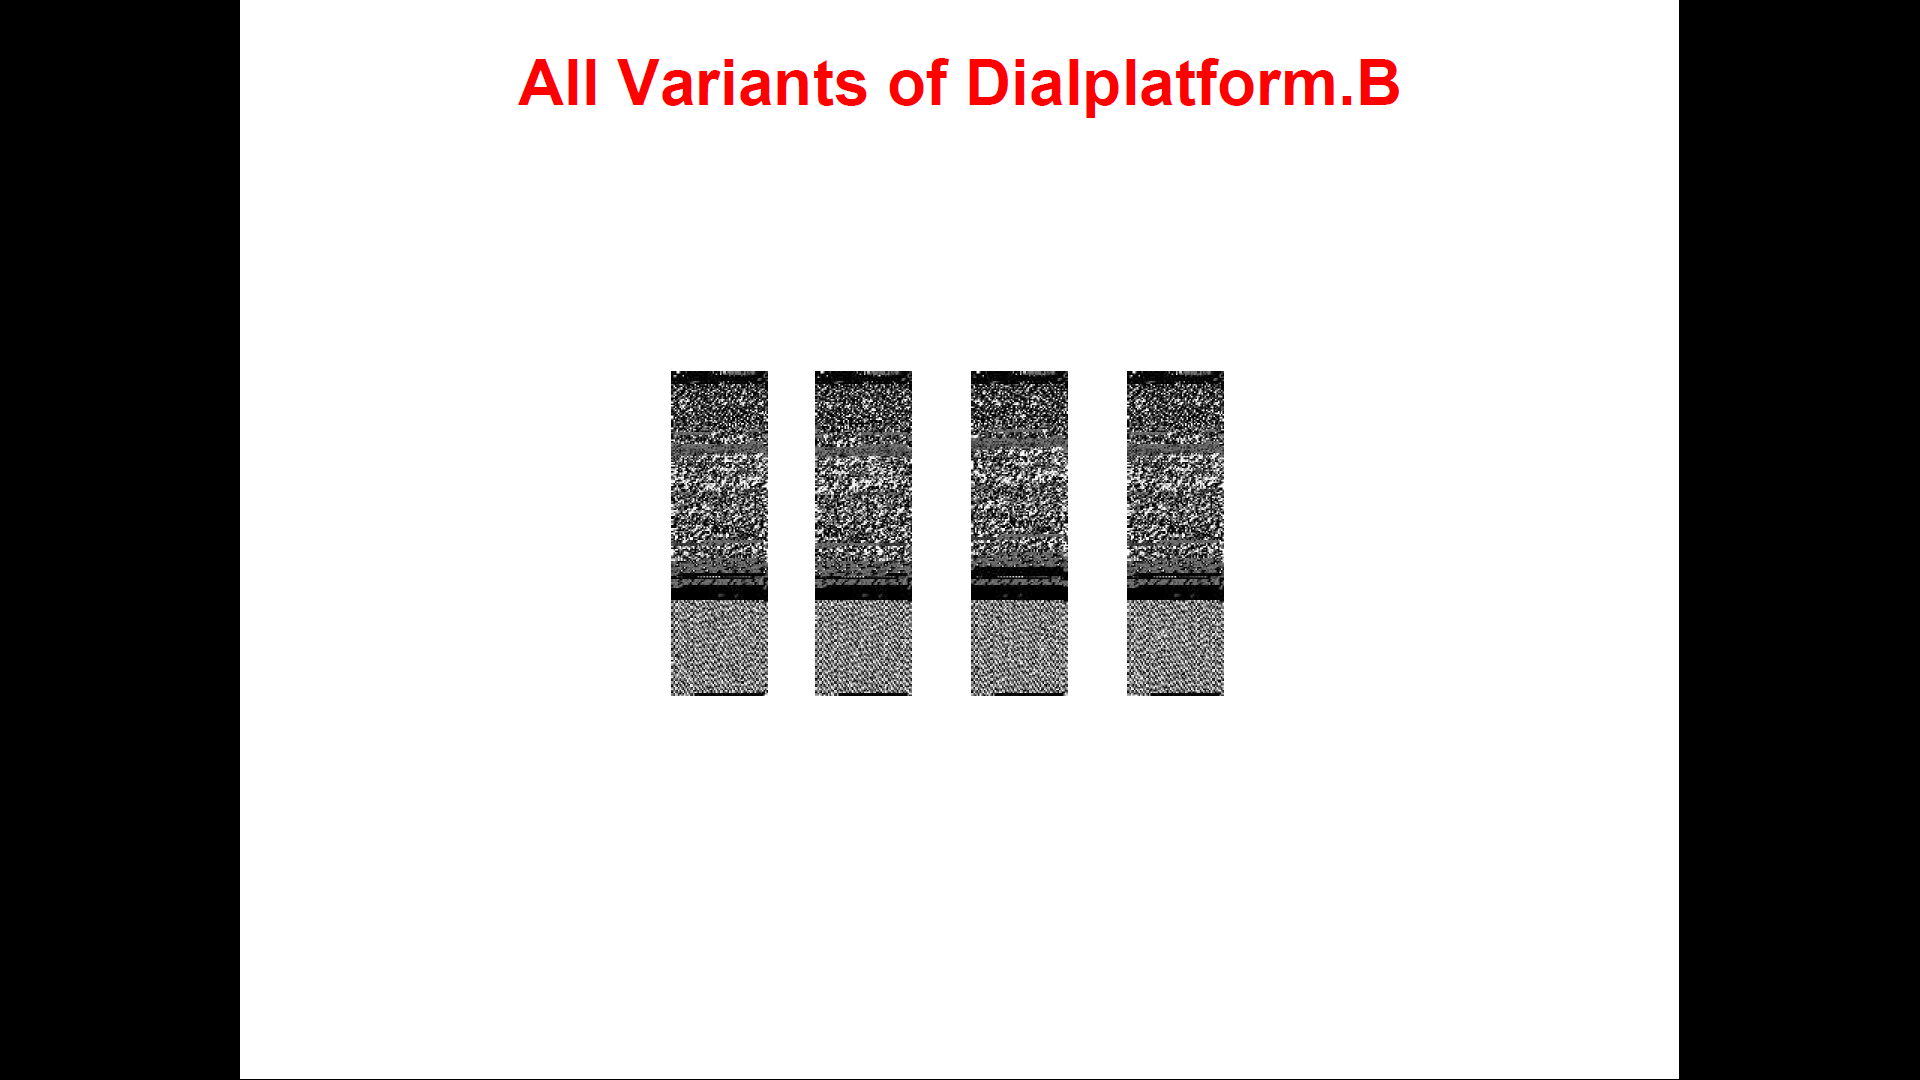
\includegraphics[width=0.80\textwidth]{images/Figure5.png}
	\captionof{figure}{All variants of the malware family Dialplatform.B.} \label{DialPlatform.BVariants}%
	\label{fig:DialPlatform.BVariants}
\end{center}
\\
\section{Evaluation of GIST descriptors on various datasets}

By using the GIST descriptor as features and running a K-Means algorithm we were able to achieve very good results with the Mallmg Dataset. The Mallmg dataset consists of 9000 malware files belonging to 25 malware families and their variants. All these malware binaries were converted to images and GIST features were extracted from them. These features were then clustered together using K-Means clustering algorithm. The average classification accuracy was 97 \%. Figure ~\ref{ConfusionMatrixAllFeatures} shows the confusion matrix for this dataset.


\begin{figure}
    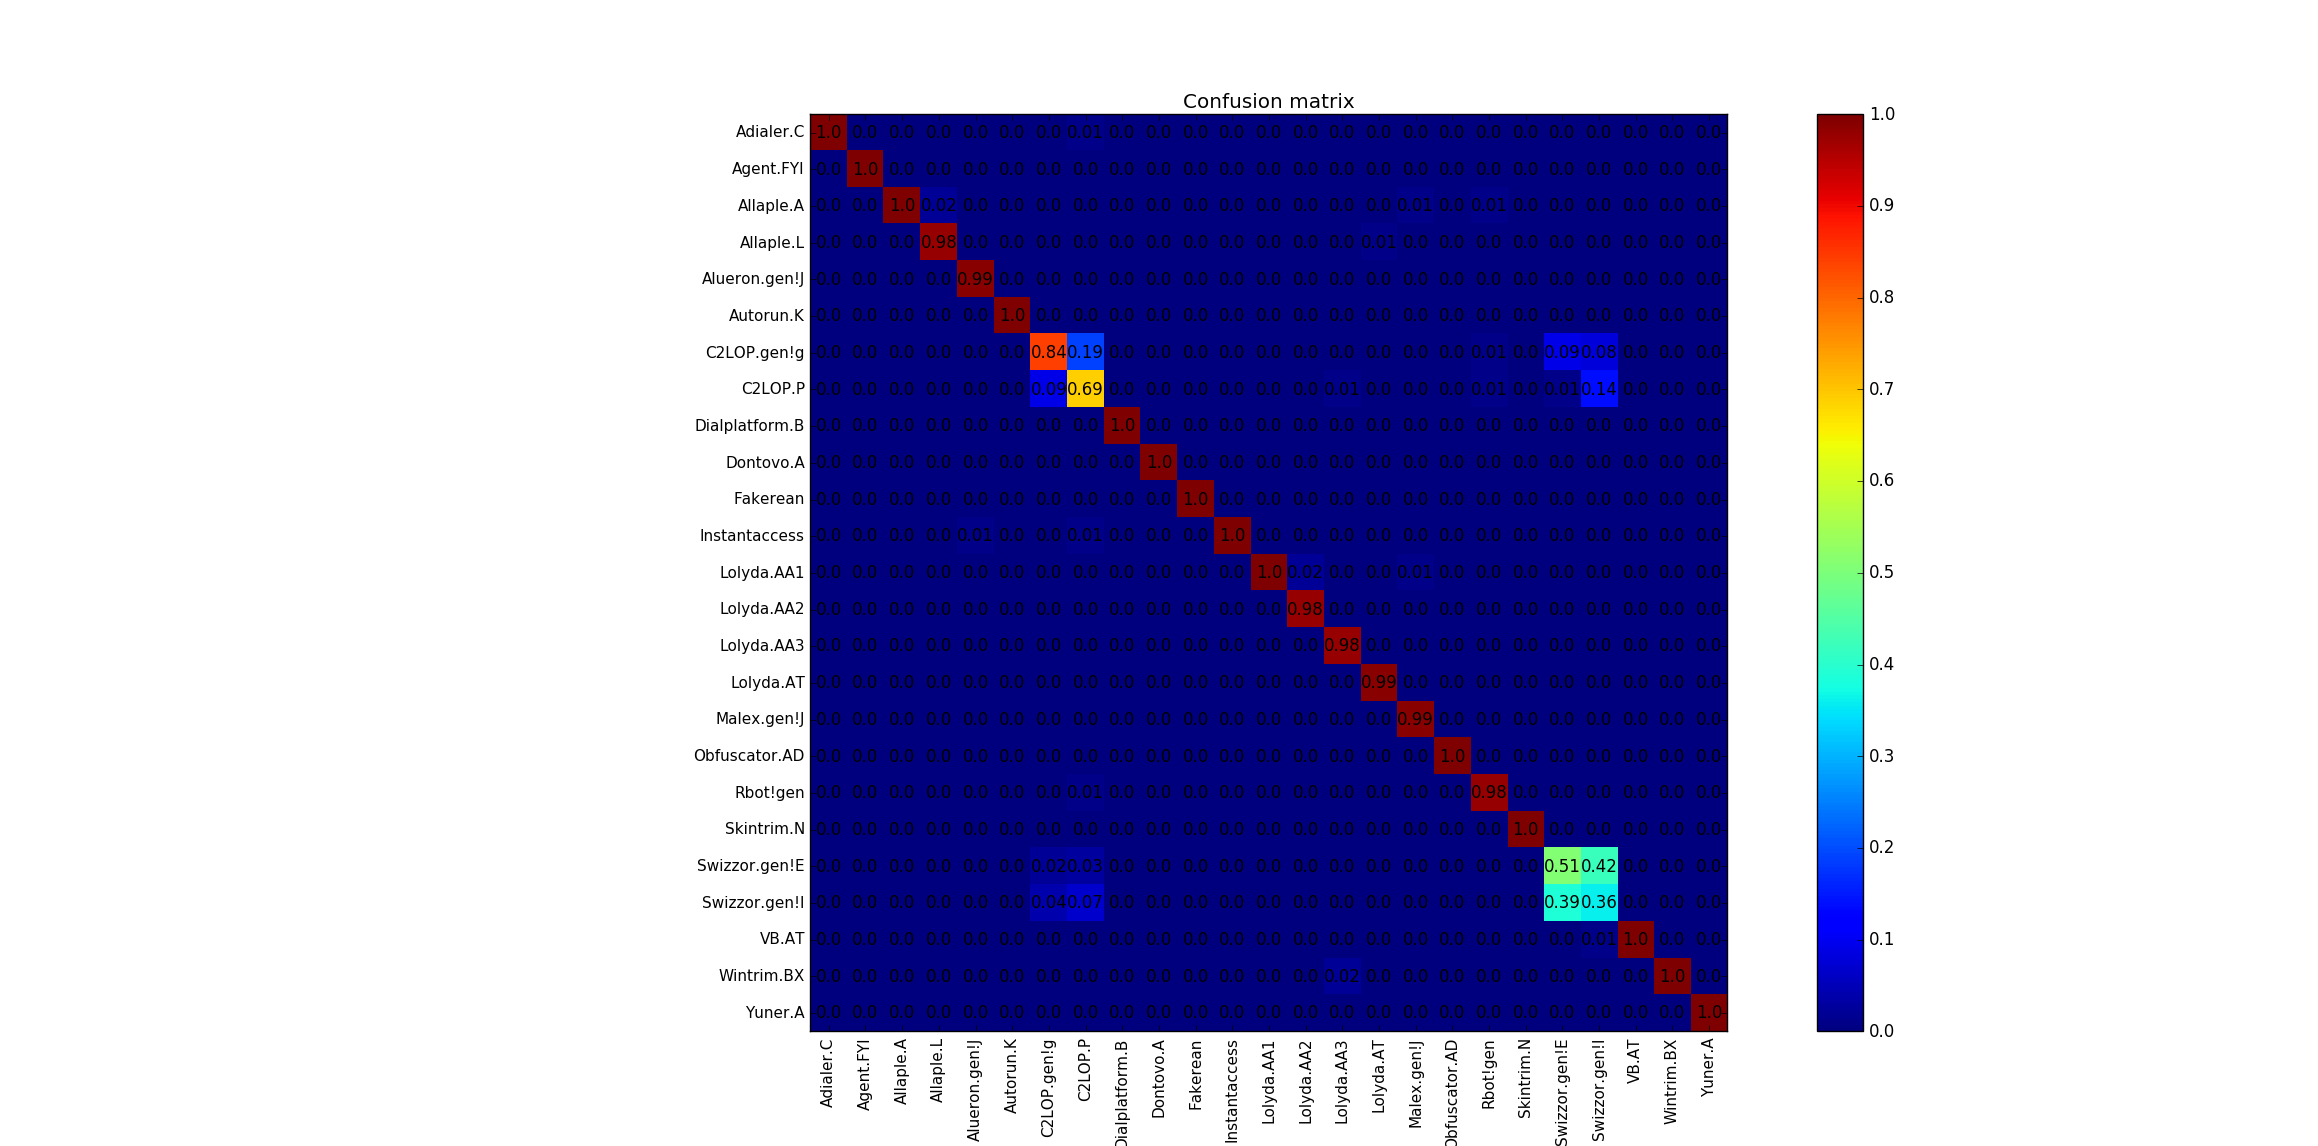
\includegraphics[width=2.0\textwidth,center]{images/Figure6_Confusion_Matrix_320_Features.png}
	\captionof{figure}{Confusion Matrix with all features.} 
	\label{ConfusionMatrixAllFeatures}%
\end{figure}


We then tested this approach with the more challenging Malicia dataset which consists primarily of ZBot, WinWebSec and ZeroAccess malware families and contains over 11000 samples. We ran the K-NearestNeighbours algorithm with 3 neighbors and achieved accuracy of over 98 \% in most cases.
\\
\section{Feature Selection}

We first used SVM Recursive Feature elimination to see when we get the best RoC for the Malicia dataset, it was found that 320 was the optimal number of features which was the same as the original number of features that were taken in to consideration. 

We then turned to Univariate feature selection from the Python Scikit package. Using this we found that even if we choose just the top 60 features we still get very good results. Univariate feature selection works by selecting the best features based on univariate statistical tests. It can be seen as a preprocessing step to an estimator. SelectKBest removes all but the k highest scoring features 
using common univariate statistical tests for each feature: false positive rate, false discovery rate, or family wise error.


Figure ~\ref{ConfusionMatrix60Features} shows the confusion matrix for Mallmg dataset with just 60 of the original number of features.

\begin{figure}
	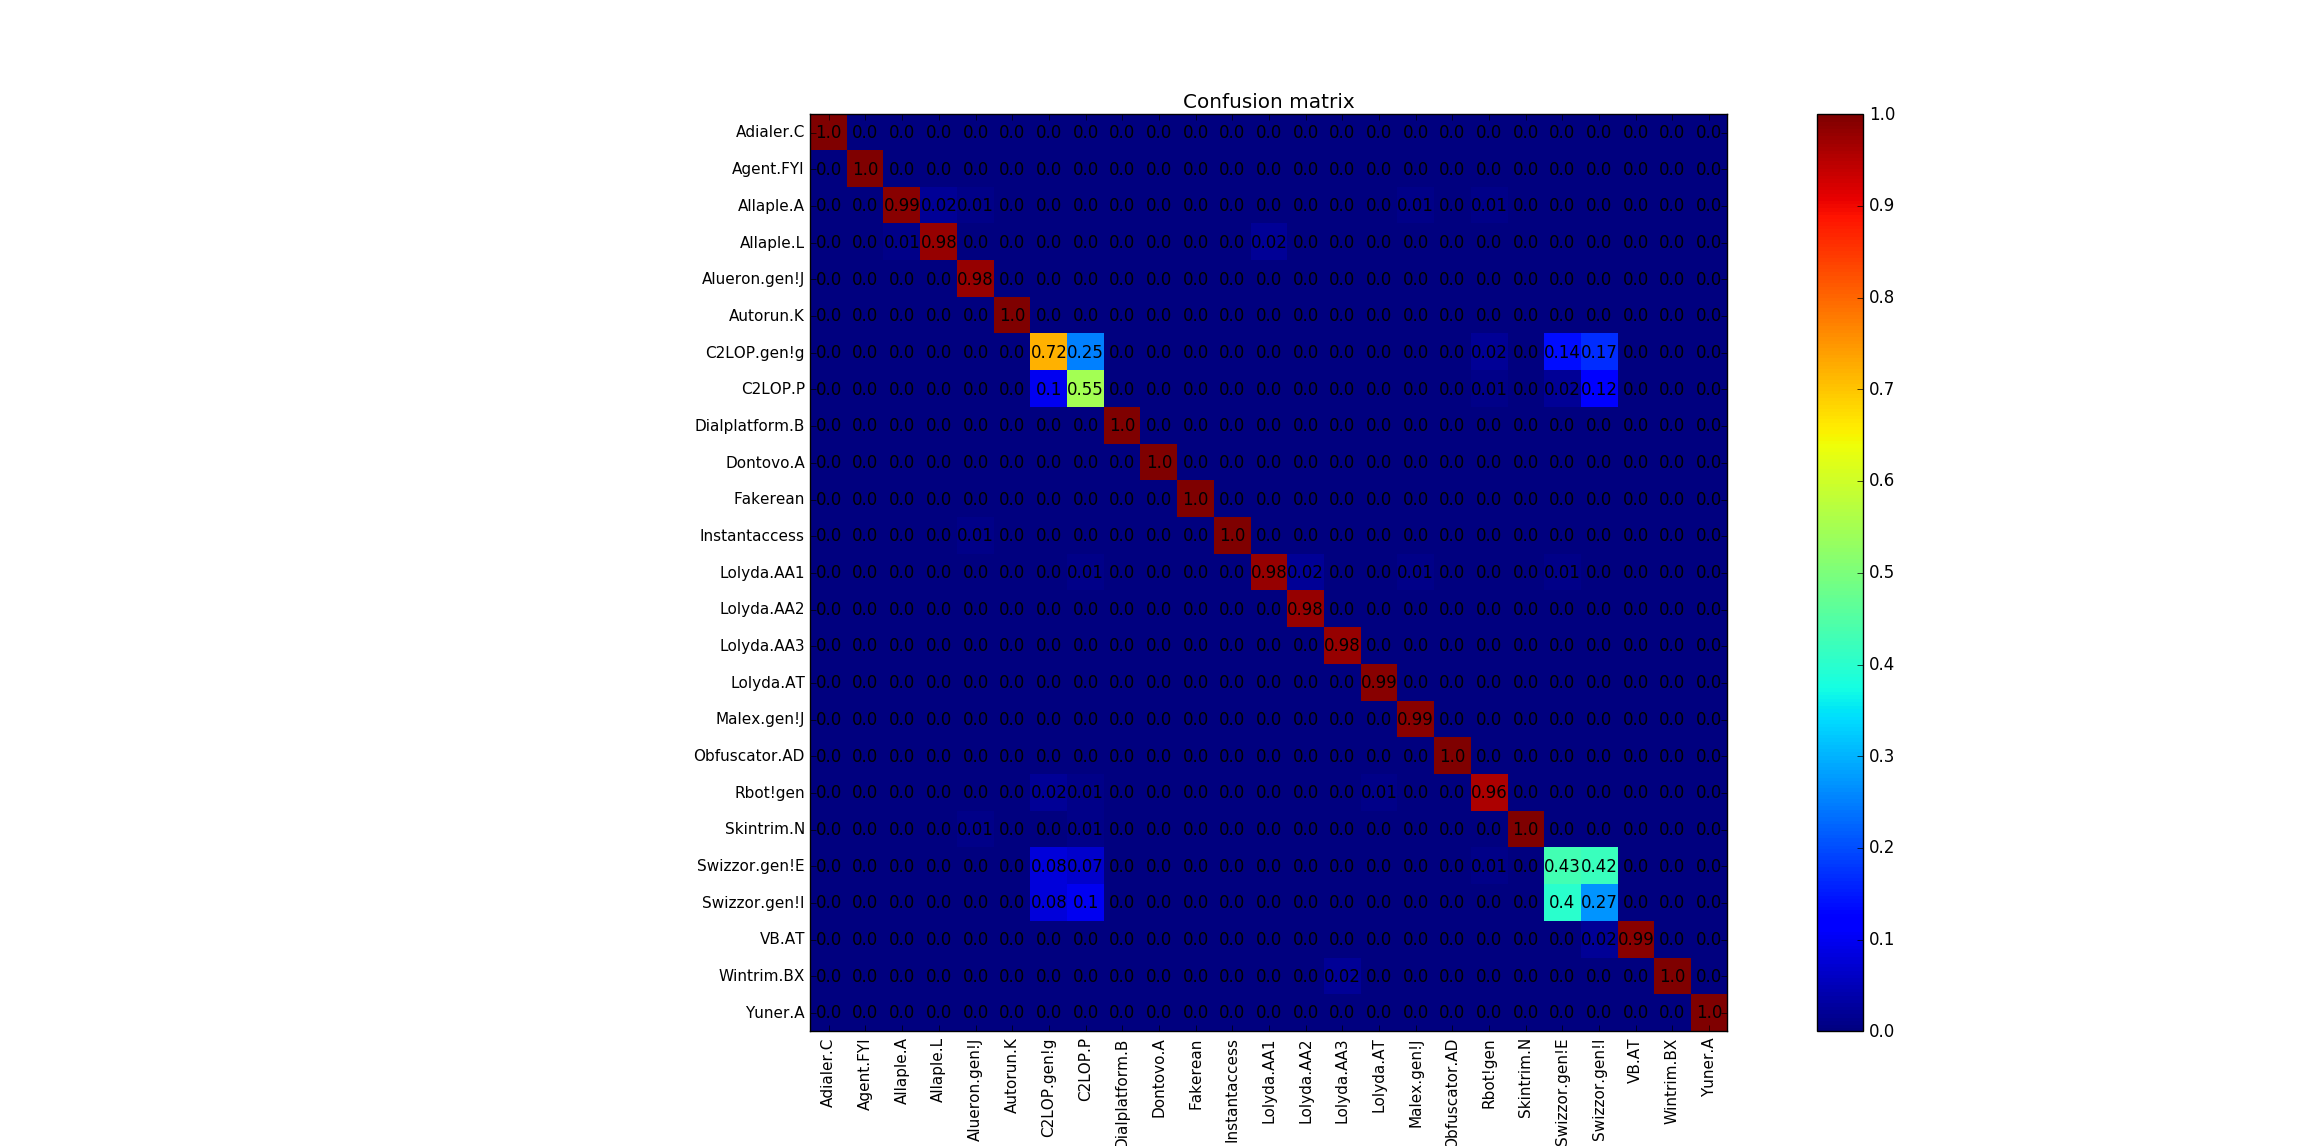
\includegraphics[width=2.0\textwidth,center]{images/Figure7_Confusion_Matrix_60_Features.png}
	\captionof{figure}{Confusion Matrix with 60 features.} 
	\label{ConfusionMatrix60Features}%
\end{figure}


Also, on the Malicia dataset we achieve 98.5 \% and 99.25 \% accuracy with 80 \% and 90 \% training data respectively.

Hence we conclude that combining univariate feature selection with GIST descriptors gives us a very good scoring algorithm which is also very efficient. 